% to compile: Shift+Alt+F1
\documentclass[a4paper,11pt]{article}%,twocolumn
%% packages

\usepackage{blindtext} % needed for creating dummy text passages
%\usepackage{ngerman} % needed for German default language
\usepackage{amsmath} % needed for command eqref
\usepackage{amssymb} % needed for math fonts
\usepackage[colorlinks=true,breaklinks]{hyperref} % needed for creating hyperlinks in the document, the option colorlinks=true gets rid of the awful boxes, breaklinks breaks lonkg links (list of figures), and ngerman sets everything for german as default hyperlinks language
\usepackage[hyphenbreaks]{breakurl} % ben�tigt f�r das Brechen von URLs in Literaturreferenzen, hyphenbreaks auch bei links, die �ber eine Seite gehen (mit hyphenation).
\usepackage{xcolor}
\definecolor{c1}{rgb}{0,0,1} % blue
\definecolor{c2}{rgb}{0,0.3,0.9} % light blue
\definecolor{c3}{rgb}{0.3,0,0.9} % red blue
\hypersetup{
    linkcolor={c1}, % internal links
    citecolor={c2}, % citations
    urlcolor={c3} % external links/urls
}
%\usepackage{cite} % needed for cite
\usepackage[square,authoryear]{natbib} % needed for cite and abbrvnat bibliography style
\usepackage[nottoc]{tocbibind} % needed for displaying bibliography and other in the table of contents
\usepackage{graphicx} % needed for \includegraphics 
\usepackage{longtable} % needed for long tables over pages
\usepackage{bigstrut} % needed for the command \bigstrut
\usepackage{enumerate} % needed for some options in enumerate
%\usepackage{todonotes} % needed for todos
\usepackage{makeidx} % needed for creating an index
\makeindex
\usepackage{gensymb}
%\usepackage{url}
\usepackage{xurl}
\usepackage{psfrag}
\usepackage{multirow}
\usepackage{subfigure}

\usepackage{algpseudocode}
\usepackage{float}
%\usepackage{minted}
\usepackage{tcolorbox}
\usepackage{menukeys}
\usepackage[
width=.8\textwidth,
justification=centering]{caption}
\usepackage{xcolor}
\usepackage{pstricks}
\usepackage{acronym}
%% page settings

\usepackage[top=20mm, bottom=20mm,left=20mm,right=20mm]{geometry} % needed for page border settings
\parindent=0mm % for space of first line of new text block
\sloppy % for writing with hyphenless justification (tries to)
\hyphenation{} % use hyphenation of tolerance parametershttp://www.jr-x.de/publikationen/latex/tipps/zeilenumbruch.html
\hyphenpenalty=10000
\exhyphenpenalty=10000
\usepackage{fancyhdr} % needed for head and foot options
%% my macros

%% Text fomats
\newcommand{\tbi}[1]{\textbf{\textit{#1}}}

% IEEE naming convention
%\renewcommand{\figurename}{Fig.}

% custom counter for shell scripts
\newcounter{shellcounter}
% \newcounter{myexample}% preamble
\newtcolorbox[
use counter=shellcounter,
number format=\Alph]{shell}[2][]{%
	colback=blue!5!white,
	colframe=blue!75!white,
	fonttitle=\bfseries,
	title= {\sc Shell \thetcbcounter}: #2,#1}


\newcounter{outputcounter}
\newtcolorbox[
use counter=outputcounter,
number format=\Roman]{result}[2][]{%
	colback=green!5!white,
	colframe=green!75!black,
	fonttitle=\bfseries,
	title= {\sc Result box \thetcbcounter}: #2,#1}


\begin{document}
\begin{titlepage}
\center % Center everything on the page

%-------------------------------------------------------------------------------------
%	HEADING SECTIONS
%------------------------------------------------------------------------------------
\textbf{\large Department of Electronic and Telecommunication Engineering}\\[0.5cm]
\textbf{\Large University of Moratuwa, Sri Lanka}\\[1cm]
\textbf{\large EN4603 - Digital IC Design}\\[2cm]

\includegraphics[width=0.3\textwidth]{figures/uomlogo}\\[2cm]

	
%-------------------------------------------------------------------------------------
%	TITLE SECTION
%------------------------------------------------------------------------------------
\textbf{\Huge Laboratory Experiment 1 \\RTL Synthesis }\\[0.2cm]
\textbf{\Large Laboratory Report}\\[3cm]


%----------------------------------------------------------------------------------------
%	MEMBERS SECTION
%----------------------------------------------------------------------------------------


\vfill

\textbf{\large Submitted by}\\[0.5cm]

\textbf{\large Submitted by}\\[2mm]
\begin{minipage}{0.3\textwidth}
	\begin{flushleft}
		{\large C.S.Pallikkonda}\\[2mm]
		{\large R.M.A.S.Rathnayake }\\[2mm]
		{\large B.P.Thalagala }\\[2mm]		
		
	\end{flushleft}
\end{minipage}
\hspace{2mm}
\begin{minipage}{0.2\textwidth}
	\begin{flushright}
		{\large 180441C }\\[2mm]
		{\large 180534N }\\[2mm]
		{\large 180631J }\\[2mm]

	\end{flushright}
\end{minipage}\\[1cm]

	
	
	
%----------------------------------------------------------------------------------------
%	DATE SECTION
%----------------------------------------------------------------------------------------

\textbf{\large Submitted on}\\[0.5cm]
\textbf{\Large \today} % Date, change the \today to a set date if you want to be precise

%----------------------------------------------------------------------------------------

\vfill % Fill the rest of the page with whitespace

\end{titlepage}

\pagebreak

\tableofcontents
\listoffigures
\listoftables
\section*{List of Abbreviations}
\addcontentsline{toc}{section}{List of Abbreviations}
\begin{acronym}
	\acro{asic}[ASIC]{Application Specific Integrated Circuit}
	\acro{atpg}[ATPG]{Automatic Test Pattern Generation}
	
	\acro{def}[DEF]{Design Exchange Format}
	\acro{dft}[DFT]{Design For Testability}
		
	\acro{gpdk}[GPDK]{Generic Process Design Kit}
		
	\acro{hdl}[HDL]{Hardware Description Language}
	
	\acro{ic}[IC]{Integrated Circuit}
		
	\acro{rtl}[RTL]{Register-Transfer Level}
	\acro{rx}[RX]{Receiver}
		
	\acro{tcl}[TCL]{Tool Command Language}
	\acro{tx}[TX]{Transmitter}
	
	\acro{uart}[UART]{Universal Asynchronous Receiver Transmitter}
	
\end{acronym}



\vfill
\begin{center}
	\textbf{\textit{*PDF is clickable}}
\end{center}

\textit{\textbf{Note:}}\\
\textit{All the materials related to the report can also be found at \url{https://github.com/bimalka98/Digital-IC-Design}}
\pagebreak


\pagebreak
\section{Introduction}

\subsection{Practical}
In this practical, we will be using \textit{Cadence Genus} to synthesize an example \ac{rtl} design, a transceiver. As inputs to Genus, we will provide

\begin{enumerate}
	\item Source Verilog files
	\item Technology libraries provided by the fabrication plant (here, $45~nm$ educational \ac{gpdk} given by Cadence) : {\tt (.lib, .lef, .tch)}
	\item Timing constraints
\end{enumerate}

and will obtain the synthesized netlist (Verilog files) and further timing constrains {\tt (.sdc)} as output. We will then analyze the area, timing and power of the synthesized design.

\subsection{RTL Synthesis}

In the context of digital hardware design, \ac{rtl} synthesis is the process of converting an \ac{rtl} description of a digital circuit into an optimized gate-level design.\\

The \ac{rtl} description of a digital circuit is written in a \ac{hdl} such as Verilog or VHDL. It specifies the digital circuit in terms of the flow of digital signals between registers, and the logical operations that are performed on those signals as they are transferred between the registers.\\

During \ac{rtl} synthesis, an \ac{rtl} compiler reads the \ac{rtl} description of the digital circuit and generates an optimized gate-level representation of the circuit. This gate-level representation is a description of the digital circuit in terms of gates and interconnections between them. Figure \ref{fig:asic_flow} illustrates an overview of an \ac{rtl} synthesis flow.


\begin{figure}[H]
	\centering
	\fbox{
		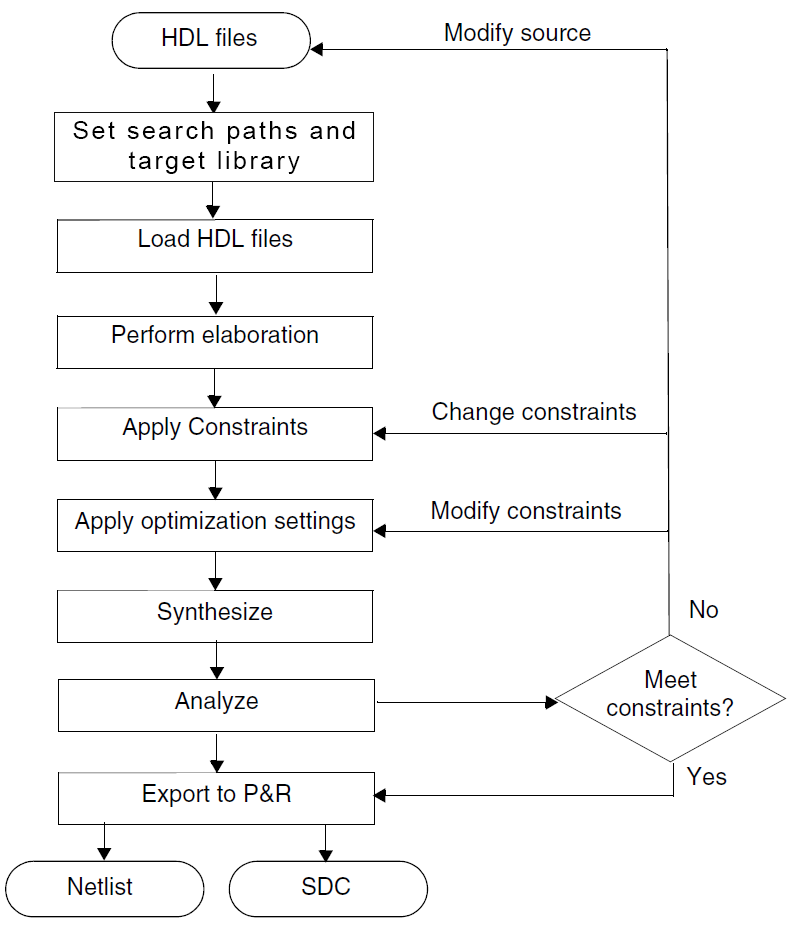
\includegraphics[width=0.53\linewidth]{figures/flow.PNG}
	}
	\caption{Overview of an \ac{rtl} synthesis flow\cite{genus_user_guide_2019}.}
	\label{fig:asic_flow}
\end{figure}

\section{Exercise}

\subsection{System Clocks \& Resets}

\subsubsection{System Clocks}





\vfill
\hrule
\vspace{0.5cm}
\bibliographystyle{IEEEtran}
\bibliography{refer}

%---------------------------------------------------------------------------
\end{document}
-
